\documentclass[../main.tex]{subfiles}

\begin{document}

\section{How Often are Recommendations Followed}
As learners engage in activities supported by a learning ecosystem, they will build
up a history of learning experiences. When the digital resources of that learning ecosystem
adhere to a framework dedicated to supporting and understanding the
learner, such as the Total Learning Architecture (TLA), it becomes
possible to retell their learning story through data and data
visualization. One important aspect of that story is the
recommendations provided to the learner and whether or not the learner
follows those recommendations.

\subsection{Ideal Statements}
In order to accurately determine if a learner is following
recommendations, there are a few requirements of the data produced by
a LRP and the recommender itself. They are as follows:
\begin{itemize}
\item Every time the recommender makes a recommendation, a statement
  should be produced which uses the verb
  $https://w3id.org/xapi/dod-isd/verbs/recommended$\footnote{\label{RecommendedIRI}
  See footnote 4} and has the
  recommended piece of content as the object.
  \begin{itemize}
    \item the content should be uniquely and consistently identified
      across all statements.
    \end{itemize}
\item When a learner launches recommended content, the resulting
  launched statement should use the verb
  $http://adlnet.gov/expapi/verbs/launched$\footnote{\label{LaunchedIRI}
  See footnote 4} and contain a refrence to the recommened content statement within
$\$.context.statement$
  \begin{itemize}
    \item Launching of content should use the above IRI regardless of
      why the content was launched
    \item If it not possible to refrence the exact recommended content
      statement, the launch statement should have some indication that
      it was the result of a recommendation.\footnote{\label{Recommendations} It is
    possible to determine if recommendations are followed (with some
    level of error) without this explicit linking of launched to
    recommended but this severly complicates the algorithm. In this
    case, in order to optmize for accuracy, the algorithm would need
    to consider the actor and their general activity within a session,
    the object of both launched and recommended statements generated
    within the session, the time lapse between recommendations and
    launches with a predefined lapse value which determines if a
    launch was close enough in time to a recommendation to be
    considered a result of the recommendation. An additonal constraint
    on the above case is the recommendation statements should contain
    a reference to to the person recieving the recommendation,
    otherwise determining the 1:1 relationships between recommendations and
    launches requires aditional complexity and will still not be 100\%
    accurate due to the reliance on the time lapse value.}
\end{itemize}
\end{itemize}

\subsection{Input Data Retrieval}
How to query an LRS via a GET request to the Statements Resource via
curl.\footnote{\label{refMoreLink2} footnote 1 applies to both S1
  and S2.}\footnote{\label{refnoZ2} See footnote
  2.}\footnote{\label{refallTime2} See footnote 3.}

\begin{lstlisting}[frame=single]
R = "verb=https://w3id.org/xapi/dod-isd/verbs/recommended"
L = "verb=http://adlnet.gov/expapi/verbs/launched"

Since = "since=2018-07-20T12:08:47Z"
Until = "until=2018-07-21T12:08:47Z"
Base = "https://example.endpoint/statements?"

endpoint1 = Base + R + "&" + Since + "&" + Until
endpoint2 = Base + L + "&" + Since + "&" + Until

Auth = Hash generated from basic auth

SR = curl -X GET -H "Authorization: Auth"
         -H "Content-Type: application/json"
         -H "X-Experience-API-Version: 1.0.3"
         endpoint1
SL = curl -X GET -H "Authorization: Auth"
         -H "Content-Type: application/json"
         -H "X-Experience-API-Version: 1.0.3"
         endpoint2

S = SR + SL
\end{lstlisting}

\subsection{Statement Parameters to Utilize}
The statement parameter locations here are written in
\href{http://goessner.net/articles/JsonPath/}{JSONPath}. This notation
is also compatable with the xAPI Z notation due to the defined
hierarchy of components. Within the Z specifications, a variable name
will be used instead of the $\$$
\begin{itemize}
\item $\$.verb.id$
\item $\$.context.statement$
\end{itemize}

\subsection{2018 Pilot TLA Statement Problems}
At the time of writing this document, launched statements do not
include a statement reference or any indication of a connection
between recommendations and launches. The authors of this document do
not have access to the LRS containing the recommended statements and
thus can not draw any conclusions about any issues which may be
present within those statements or any aspects of those statements
which may correlate them to launch statements. The following algorithm
is going to assume that the input set of statements follow the
guidlines outlined in section 5.1 as the additional algorithmic
considerations brought on by non ideal statements, as specified within
footnote 16, result in an algoirthm which is not optimal for near real
time visualizations.

\subsection{Summary}
\begin{enumerate}
  \item Query an LRS via a GET request to the statements endpoint
    using the paramters verb, since and until to gather all statements
    with the verb $http://adlnet.gov/expapi/verbs/launched$.
  \item Query an LRS via a GET request to the statements endpoint
    using the paramters verb, since and until to gather all statements
    with the verb $https://w3id.org/xapi/dod-isd/verbs/recommended$.\footnote{\label{sameSession} If since and until are specified,
      they should be the same in both requests.}
  \item Group all collections of statements by a $TIMEUNIT$
  \item seperate the collection of grouped launched statements into a
    collection of those which were the result of a recommendation and
    those which were not.
  \item Take the count of all groups of statements
    \begin{itemize}
    \item Recommended statements per $TIMEUNIT$
    \item Launches due to recommendations per $TIMEUNIT$
    \item Launches not due to recommendations per $TIMEUNIT$
    \end{itemize}
  \item Calculate summary statistics for the overall time range and
    per $TIMEUNIT$
    \begin{itemize}
    \item Divide launches due to recommendations by the total number of
      launches to determine the percentage of launches due to
      recommendations
    \item Divide launches due to recommendations by the total number
      of recommendations to determine the percentage of
      recommendations which are followed.
    \end{itemize}
\end{enumerate}

$\\\\$

\subsection{Formal Specification}

\subsubsection{System State}

\begin{schema}{FollowedRecommendations}
  Statements \\
  CountPerGroup \\
  S_{recommended},S_{launched} : \finset_1 \\
  ordered_{L}, ordered_{R}, grouped_{launched}, grouped_{recommended}, \\
  onlyRecommended, cPerGroup_{launched}, cPerGroup_{recommended}, \\
  cPerGroup_{followed}, combined : \seq \\
  t_{start}, N_{launched}, N_{recommended}, N_{followed}, P_{followed}, P_{dueto}  : \nat \\
  tr_{start}, tr_{end} : \finset \\
  unit? : TIMEUNIT
  \where
  S_{recommended} = statements \\
  S_{launched} = statements \\
  combined = \langle (tr_{start}, tr_{end}, N_{launched}, N_{recommended},
  N_{followed}, P_{followed}, P_{dueto})\rangle \\
  count(grouped_{launched}) = count(grouped_{recommended}) \\
  count(onlyRecommended) = count(grouped_{launched}) \implies \\
  count(onlyRecommended) = count(grouped_{recommended}) \\
  count(cPerGroup_{launched}) = count(cPerGroup_{followed}) = count(cPerGroup_{recommended})
\end{schema}

\begin{itemize}
\item $S_{recommended}, S_{launched}$ are both non-empty, finite sets.
  \begin{itemize}
  \item $S_{recommended}$ and $S_{launched}$ contain
    the results of querying an LRS for recommended and launched
    statements respectively.
  \end{itemize}
\item $ordered_{L}, ordered_{R}, grouped_{launched},
  grouped_{recommended},$ $onlyRecommended, \\ cPerGroup_{launched},
  cPerGroup_{recommended}, cPerGroup_{followed}$ and $combined$ are
  all finite sequences.
  \begin{itemize}
    \item $ordered_{L}$ and $ordered_{R}$ are the sequences of
      statements within $S_{launched}$ and $S_{recommended}$
      respectively and sorted by timestamp.
    \item $grouped_{launched}$ is the result of grouping the
      statements within $ordered_{L}$ by $unit?$.
    \item $grouped_{recommended}$ is the result of grouping the
      statements within $ordered_{R}$ by $unit?$.
    \item $onlyRecommended$ is the result of filtering the statements
      within the sequence $grouped_{launched}$ to only include
      statements where $statement.context.statement$ is present
    \item $cPerGroup_{launched}, cPerGroup_{recommended},
      cPerGroup_{followed}$ are all sequences of numbers which
      represent the count within each subsequence of
      $grouped_{launched}$, $grouped_{recommended}$ and
      $onlyRecommended$ respectively.
    \item $combined$ is a sequence of ordered pairs where each pair
      consists of $tr_{start}$, $tr_{end}$, $N_{launched}$,
      $N_{recommended}$, $N_{followed}$, $P_{followed}$ and $P_{dueto}$
    \end{itemize}
\item $t_{start}, N_{launched}, N_{recommended}, N_{followed},
  P_{followed}, P_{dueto}$ are all natural numbers
\item $tr_{start}, tr_{end}$ are both timestamps which represent the
  the start and end of the time range for each a group of statements.
\item $unit?$ is an input representing a time interval, ie day vs
  month vs hour.
\item all sequences are the same length so that each subsequence
  represents the same time grouping. In other words, indexes are
  comparable across sequences.
\end{itemize}

\subsubsection{Initial System State}

\begin{schema}{InitFollowedRecommendations}
  FollowedRecommendations \\
  \where
  S_{recommended} \not = \emptyset \\
  S_{launched} \not = \emptyset \\
  unit? = \{day\} \\
  ordered_{L} = \langle  \rangle \\
  ordered_{R} = \langle  \rangle \\
  grouped_{launched} = \langle  \rangle \\
  grouped_{recommended} = \langle  \rangle \\
  onlyRecommended = \langle  \rangle \\
  cPerGroup_{launched} = \langle  \rangle \\
  cPerGropu_{recommended} = \langle  \rangle \\
  cPerGroup_{followed} = \langle  \rangle \\
  combined = \langle  \rangle \\
  t_{start} = 0 \\
  N_{launched} = 0 \\
  N_{recommended} = 0 \\
  N_{followed} = 0 \\
  P_{followed} = 0 \\
  P_{dueto} = 0 \\
\end{schema}

\begin{itemize}
  \item $S_{recommended}$ and $S_{launched}$ are initially not empty
    sets
  \item all sequences are initially empty
  \item all numbers are initially zero
  \item the default $TIMEUNIT$ is set to day
\end{itemize}

\subsubsection{Group by Timestamp}

\begin{schema}{SortByTimestamp}
  Statement \\
  IsoToUnix \\
  orderByTimestamp : \finset_1 \fun seq_1 \\
  o? : \finset_1 \\
  o! : seq_1 statement
  \where
  o? = \{o : statement\} \\
  o! = orderByTimestamp(o?) \\
  o! = \langle o_{i}..o_{j} \rangle @ \forall o_{n} : o_{i}..o_{j} @
  o_{n} : STATEMENT \land i \leq n \leq j @ \\\t3
  convert(o_{i}.timestamp) \leq convert(o_{n}.timestamp) \leq
  convert(o_{j}.timestamp)
\end{schema}

\begin{itemize}
\item The schema $SortByTimestamp$ introduces the function
  $orderByTimestamp$ which takes in a non-empty, finite set and
  returns a non-empty, finite sequence.
\item $orderByTimestamp$ is a sequence of statements ordered from
  earliest to latest.
\end{itemize}

\begin{schema}{WithinRange}
  withinRange : (\nat, \nat, \nat, TIMEUNIT) \fun \finset_1\#1 \\
  in?, start?, state? : \nat \\
  unit? : TIMEUNIT \\
  out! : \{TRUE\} \lor \{FALSE\}
  \where
  unit? \, = \,\{second\} \implies 1 \lor \{minute\} \implies 60
  \lor \{hour\} \implies 3600 \,\lor \\\t2 \{day\} \implies 86400 \lor
  \{week\} \implies 604800 \,\lor \\\t2 \{month\} \implies 2629743
  \lor \{year\} \implies 31556926 \\

  out! = withinRange(in?, start?, state?, unit?) \\
  withinRange(in?, start?, state?, unit?) = \\\t3 \IF in? \leq
  start? + ((state? + 1) * unit?) \\\t4 \THEN out! = \{TRUE\} \\\t4 \ELSE
  out! = \{FALSE\} \\
\end{schema}

\begin{itemize}
\item The schema $WithinRange$ introduces the function $withinRange$
  which takes in three numbers and a $TIMEUNIT$ and returns either
  $\{TRUE\}$ or $\{FALSE\}$
\item $withinRange$ checks to see if $in?$ is less than or equal to a
  start time $start?$ plus the result of multiplying the numeric
  conversion for $unit?$ by the $state?$.
\item $state?$ represents the current group, ie. day 1 vs day 2 vs day
  3. The $+ 1$ is to account for array indexes starting at 0.
\end{itemize}

\begin{schema}{GroupByTimeUnit}
  Statement \\
  IsoToUnix \\
  WithinRange \\
  groupByTimeUnit : (\seq_1, \nat, TIMEUNIT) \fun \seq_1 \\
  g?,g! : \seq_1 \\
  t_{start}? : \nat
  \where
  g? = \langle g?_{i}..g?_{j} \rangle @ \forall g?_{n} :
  g?_{i}..g?_{j} @ i \leq n \leq j @ g?_{n} = statement \,\land \\\t1
  convert(g?_{i}.timestamp) \leq convert(g?_{n}.timestamp) \leq
  convert(g?_{j}.timestamp) \\
  g! = groupByTimeUnit(g?, t_{start}? state?, unit?) \\
  g! = \langle g : seq \,|\, \forall g?_{n} :
  g?_{i}..g?_{j} @
  \exists_1 \langle g_{r} \rangle : \langle g_{q} \rangle
  .. \langle g_{s} \rangle @ q \leq r \leq s \land r = state? @
  \\\t3 \IF withinRange(convert(g?_{n}.timestamp), t_{start}, r, unit?) =
  \{TRUE\} \\\t4 \THEN g? \extract g?_{n} \,\land\, g?_{n} \inseq
  \langle g_{r} \rangle \implies \langle g_{r} \rangle = \langle
  g_{ri}..g_{rn}..g_{rj} \rangle @ ri \leq rn \leq rj @ g_{rn} =
  g?_{n}  \\\t4 \ELSE \IF \forall g_{n}? : g_{i}?..g_{j}? @
  withinRange(g?_{n}, t_{start}, r, unit?) = \{FALSE\} \\\t5 \THEN
  groupByTimeUnit((g? \extract \langle g_{r} \rangle) , t_{start}? (r
  + 1), unit?) @ \langle g_{r} \rangle = \langle  \rangle \, \lor \not
  = \langle  \rangle \rangle
\end{schema}

\begin{itemize}
\item The schema $GroupByTimeUnit$ intorudces the function
  $groupByTimeUnit$ which takes as arguments a non-empty, finite
  sequence, a natural number and a $TIMEUNIT$ and outputs a non-empty,
  finite sequence of sequences.
\item For every statement within the input sequence, $groupByTimeUnit$
  checks to see if the timestamp of that statement is within the range
  of $t_{start}$ and $unit?$. If it is, that statement is removed from
  the input sequence $g?$ and added to the current subsequence
  $\langle g_{r} \rangle$. If none of the remaining statements within
  the input sequence are within the range of $t_{start}$ and $unit?$,
  then the variable $state?$ is incremented, the current subsequence
  $\langle g_{r} \rangle$ is either a collection of matched statements or is an
  empty sequence and the search for remaining subsequences $\langle
  g_{r+state?} \rangle$ continues.
\item because the input sequence $g?$ is orderd chronologically, this
  implies that once a statement does not fit into a range, the rest of
  the statements remaining in the input sequence will not fit into
  that range and $state?$ must be incremented to generate a new
  subsequence $\langle g_{r + state?} \rangle$ so that the remaining
  statements can be grouped.
\end{itemize}
$\\\\\\\\\\\\\\\\$ %header with text
\subsubsection{Processes Results}

\begin{schema}{OrderStatements}
  \Delta FollowedRecommendations \\
  SortByTimestamp
  \where
  ordered_{L}' = orderByTimestamp(S_{launched}) \\
  ordered_{R}' = orderByTimestamp(S_{recommended}) \\
  t_{start}' = convert((head~ordered_{L}').timestamp) \\
\end{schema}

\begin{itemize}
  \item The schema $OrderStatements$ updates the system state defined
    by the schema $FollowedRecommendations$.
  \item $ordered_{L}'$ is the result of ordering the statements contained
    within the set $S_{launched}$ chronologically.
  \item $ordered_{R}'$ is the result of ordering the statements contained
    within the set $S_{recommended}$ chronologically.
  \item $t_{start}'$ is the timestamp from the first statement within
    $ordered_{L}'$ converted to unix time.
\end{itemize}

\begin{schema}{GroupByTime}
  \Delta FollowedRecommendations \\
  GroupByTimeUnit \\
  \where
  grouped_{launched}' = groupByTimeUnit(ordered_{L}', t_{start}', 0, unit?) \\
  grouped_{recommended}' = groupByTimeUnit(ordered_{R}', t_{start}',
  0, unit?)
\end{schema}

\begin{itemize}
  \item The schema $GroupByTime$ updates the state defined by the schema
    $FollowedRecommendations$.
  \item $grouped_{launched}'$ is the result of passing $ordered_{L}'$,
    $t_{start}'$, 0 and $unit?$ to the function $groupByTimeUnit$.
  \item $grouped_{recommended}'$ is the result of passing $ordered_{R}'$,
    $t_{start}'$, 0 and $unit?$ to the function $groupByTimeUnit$.
\end{itemize}

\begin{schema}{OnlyRecommendedLaunches}
  \Delta FollowedRecommendations
  \where
  onlyRecommended' = \langle o : seq \,|\, \LET grouped_{launched}'==gl
  \implies \\\t5 \langle \langle gl_{i} \rangle..\langle gl_{j}
  \rangle \rangle \implies \langle \langle gl_{ii}..gl_{ij}
  \rangle..\langle gl_{ji}..gl_{jj}\rangle\rangle @ \\\t5
  \forall \langle gl_{n} \rangle : \langle gl_{i} \rangle..\langle
  gl_{j} \rangle @ \exists_1 \langle o_{n} \rangle : \langle o_{i}
  \rangle..\langle o_{j} \rangle \implies \langle \langle o_{ii}..o_{ij} \rangle..\langle
  o_{ji}..o_{jj}\rangle\rangle @ \\\t5 ((\forall o_{in} : o_{ii}..o_{ij} @
  o_{in}.context.statement \not = \emptyset \land o_{in} \inseq
  gl_{i}) \land \\\t5 (\forall o_{jn} : o_{ji}..o_{jj} @
  o_{jn}.context.statement \not = \emptyset \land o_{jn} \inseq
  gl_{j})) \lor \\\t5 \langle o_{n} \rangle = \langle \rangle \rangle \\
\end{schema}

\begin{itemize}
  \item The schema $OnlyRecommendedLaunches$ updates the state defined
    by the schema $FollowedRecommendations$.
  \item $onlyRecommended'$ is the sequence of objects $o$ where $o$ is
    a sequence consisting of statements (or no statements) from the corresponding sequences
    within  $grouped_{launched}'$ where $statement.context.statement$
    exists.
  \item $onlyRecommended'$ maintains the same number and ordering of time groups
    (subsequences) as $grouped_{launched}'$ and
    $grouped_{recommended}'$.
\end{itemize}

\begin{schema}{GetCounts}
  \Delta FollowedRecommendations \\
  CountPerGroup
  \where
  cPerGroup_{launched}' = \langle c : \nat \,|\, \LET grouped_{launched}'==gl \implies
  \langle \langle gl_{i} \rangle..\langle gl_{j} \rangle \rangle @ \\\t5
  \forall \langle gl_{n} \rangle : \langle gl_{i} \rangle..\langle gl_{j} \rangle @
  \exists_1 c_{n} : \nat @ \\\t5 \IF gl_{n} = \langle \rangle \\\t6 \THEN c_{n} =
  0 \\\t6 \ELSE c_{n} = count(\langle gl_{n} \rangle)
  \rangle \\
  cPerGroup_{recommended}' = \langle c : \nat \,|\, \LET grouped_{recommended}'==gr \implies
  \langle \langle gr_{i} \rangle..\langle gr_{j} \rangle \rangle @ \\\t6
  \forall \langle gr_{n} \rangle : \langle gr_{i} \rangle..\langle gr_{j} \rangle @
  \exists_1 c_{n} : \nat @ \\\t6 \IF gr_{n} = \langle \rangle \\\t7 \THEN c_{n} =
  0 \\\t7 \ELSE c_{n} = count(\langle gr_{n} \rangle)
  \rangle \\
  cPerGroup_{followed}' = \langle c : \nat \,|\, \LET
  onlyRecommended'==or \implies \langle \langle or_{i} \rangle..\langle or_{j} \rangle \rangle @ \\\t5
  \forall \langle or_{n} \rangle : \langle or_{i} \rangle..\langle or_{j} \rangle @
  \exists_1 c_{n} : \nat @ \\\t5 \IF or_{n} = \langle \rangle \\\t6 \THEN c_{n} =
  0 \\\t6 \ELSE c_{n} = count(\langle or_{n} \rangle) \rangle \\
\end{schema}

\begin{itemize}
  \item The schema $GetCounts$ updates the state defined by the schema
    $FollowedRecommednations$.
  \item $cPerGroup_{launched}'$ is a sequence of numbers $c$ where
    each $c$ is either 0 or the result of passing the current
    subsequence of $grouped_{launched}'$ ($gl_{n}$) to the function
    $count$.
  \item  $cPerGroup_{recommended}'$ is a sequence of numbers $c$ where
    each $c$ is either 0 or the result of passing the current
    subsequence of $grouped_{recommended}'$ ($gr_{n}$) to the function
    $count$.
  \item  $cPerGroup_{followed}'$ is a sequence of numbers $c$ where
    each $c$ is either 0 or the result of passing the current
    subsequence of $onlyRecommended'$ ($or_{n}$) to the function
    $count$.
\end{itemize}

\begin{schema}{CombineSequences}
  \Delta FollowedRecommendations
  \where
  combined' = \langle c : (tr_{start}', tr_{end}', N_{launched}',
  N_{recommended}', N_{followed}', P_{followed}', P_{dueto}') \,|\, \\\t3
  \LET grouped_{launched}'==gl \implies \langle \langle gl_{i}
  \rangle..\langle gl_{n} \rangle .. \langle gl_{j} \rangle \rangle \\\t3\:\:\:\:\:\:\:
  cPerGroup_{launched}'==cl \implies \langle cl_{i}..cl_{n}..cl_{j} \rangle \\\t3\:\:\:\:\:\:\:
  cPerGroup_{recommended}'==cr \implies \langle cr_{i}..cr_{n}..cr_{j} \rangle \\\t3\:\:\:\:\:\:\:
  cPerGroup_{followed}'==cf \implies \langle cf_{i}..cf_{n}..cf_{j} \rangle \\\t3
  @ \forall \langle gl_{n} \rangle : \langle gl_{i} \rangle..\langle
  gl_{j} \rangle @ i \leq n \leq j @
  \\\t3 \exists_1 \, c_{n} : (tr_{startn}, tr_{endn}, N_{launchedn},
  N_{recommendedn}, N_{followedn}, P_{followedn}, P_{dueton}) @
  \\\t3 tr_{startn} = (head~gl_{n}).timestamp
  \\\t3 tr_{endn} = (last~gl_{n}).timestamp
  \\\t3 N_{launchedn} = cl_{n}
  \\\t3 N_{recommendedn} = cr_{n}
  \\\t3 N_{followedn} = cf_{n}
  \\\t3 P_{followedn} = cf_{n} \div cr_{n}
  \\\t3 P_{dueton} = cf_{n} \div cl_{n} \rangle
\end{schema}

\begin{itemize}
  \item The schema $CombineSequences$ changes the state defined by the
    schema $FollowedRecommendations$.
  \item $combined'$ is a sequence of objects $c$ where each $c$ is an
    ordered pair of $tr_{start}', tr_{end}', N_{launched}',
    N_{recommended}', N_{followed}', P_{followed}', P_{dueto}'$.
  \item for each $c_{n}$:
    \begin{itemize}
    \item  $tr_{start}' \bind tr_{startn}$ which is equal to the
      timestamp for the first statement within $gl_{n}$
    \item $tr_{end}' \bind tr_{endn}$ which is equal to the timestamp
      for the last statement within $gl_{n}$.
    \item $N_{launched}' \bind N_{launchedn}$ which is equal to the
      current count of launched statements within the nth time
      grouping aka $cl_{n}$.
    \item $N_{recommended}' \bind N_{recommendedn}$ which is equal to
      the current count of recommended statements within the nth time
      grouping aka $cr_{n}$.
    \item $N_{followed}' \bind N_{followedn}$ which is equal to the
      current count of recommended statements within the nth time
      grouping aka $cf_{n}$.
    \item $P_{followed}' \bind P_{followedn}$ which is equal to the
      result of dividing $cf_{n}$ by $cr_{n}$.
    \item $P_{dueto}' \bind P_{dueton}$ which is equal to the result
      of dividing $cf_{n}$ by $cl_{n}$.
    \end{itemize}
  \end{itemize}

\subsubsection{Sequence of Operations}
  $ProcessFollowedRecommendations \defs \\ OrderStatements \semi
  GroupByTime \semi OnlyRecommendedLaunches \semi \\ GetCounts \semi
  CombineSequences$
\begin{itemize}
\item The schema $ProcessFollowedRecommendations$ defines the order of
  operations for the steps within the $FollowedRecommendations$ algorithm.
\end{itemize}

\subsubsection{Return}

\begin{schema}{ReturnFollowedRecommendations}
  \Xi FollowedRecommendations \\
  ProcessFollowedRecommendations \\
  combined! : \seq
  \where
  combined! = combined'
\end{schema}

\begin{itemize}
  \item The schema $ReturnFollowedRecommendations$ describes the return
    value of the system defined by the schema
    $FollowedRecommendations$
  \item The return value $combined!$ is the variable $combined'$
    defined wtihin the schema $CombineSequences$
\end{itemize}

\subsection{Pseudocode}

\begin{algorithm}[H]
  \SetAlgoLined
  \KwIn{$S_{recommended}$, $S_{launched}$ $timeUnit$}
  \KwResult{$combined'$}
  $ordered_{L}' \leftarrow orderByTimestamp(S_{launched})$; \\
  $ordered_{R}' \leftarrow orderByTimestamp(S_{recommended})$; \\
  $t_{start}' \leftarrow convert((head~ordered_{L}').timestamp)$;\\
  $grouped_{launched}' \leftarrow groupByTimeUnit(ordered_{L}',
   t_{start}', 0, timeUnit)$;\\
  $grouped_{recommended}' \leftarrow groupByTimeUnit(ordered_{R}',
   t_{start}', 0, timeUnit)$;\\
  $grouped_{followed} \leftarrow []$;\\
   \ForEach{$G \inseq grouped_{launched}'$}
   {$curGrouping \leftarrow []$;\\
     \ForEach{$G_{n} \inseq G$}
     {\eIf{$G_{n}.context.statement \not = nil$}
       {\bf do \\
         $curGrouping' \leftarrow curGrouping \cat G_{n}$;\\
         recur curGrouping'}
       {\bf recur curGrouping'}}
   {\bf $grouped_{followed}' \leftarrow grouped_{followed} \cat
   curGrouping'$;\\
   recur $grouped_{followed}'$}}
   $C_{launched} \leftarrow {\bf map \, count() \,
     grouped_{launched}'}$;\\
   $C_{recommended} \leftarrow {\bf map \, count() \,
     grouped_{recommended}'}$;\\
   $C_{followed} \leftarrow {\bf map \, count() \,
     grouped_{followed}'}$;\\
   $combined \leftarrow []$;\\
   \For{$i\gets0$ \KwTo $count(c_{launched})$ \KwBy $1$}{
     $tr_{starti} \leftarrow (first(nth(grouped_{launched}',
     i))).timestamp$;\\
     $tr_{endi} \leftarrow (last(nth(grouped_{launched}',
     i))).timestamp$;\\
     $N_{Li} \leftarrow nth(C_{launched}, i)$;\\
     $N_{Ri} \leftarrow nth(C_{recommended}, i)$;\\
     $N_{Fi} \leftarrow nth(C_{followed}, i)$; \\
     $P_{Fi} \leftarrow N_{fi} \div N_{Ri}$;\\
     $P_{duetoi} \leftarrow N_{fi} \div N_{Li}$;\\
     $subVec_{i} \leftarrow [tr_{starti}, tr_{endi}, N_{Li}, N_{Ri},
     N_{Fi}, P_{Fi}, P_{duetoi}]$;\\
     $combined' \leftarrow combined \cat subVec_{i}$}
   \Return $combined'$
  \caption{Followed Recommendations}
\end{algorithm}
\begin{itemize}
\item {\bf map count() $grouped_{...}'$} means apply the function {\bf
  count()} to every sequence within the sequence $grouped_{...}$ and
put all results into a single array.
\end{itemize}

\subsection{JSON Schema}
\begin{lstlisting}[]
{"type":"array",
   "items":{"type":"array",
      "items":[{"type":"string"}, {"type":"string"},
               {"type":"number"}, {"type":"number"},
               {"type":"number"}, {"type":"number"},
               {"type":"number"}]}}
\end{lstlisting}
\subsection{Visualization Description}

The {\bf Followed Recommendations} visualization can be a bar chart
where the domain is time ranges and the range is a number
representing the total count of statements recorded. For each time
range, there will be three groups: 1) the number of launched
statements 2) the number of recommended statements 3) the number of
launches which are due to recommendations. Above each grouping or on
hover, summary statistics can be desplayed which describe the
percentage of launches due to recommendations and the percentage of
recommendations which were followed.

\subsection{Visualization prototype}

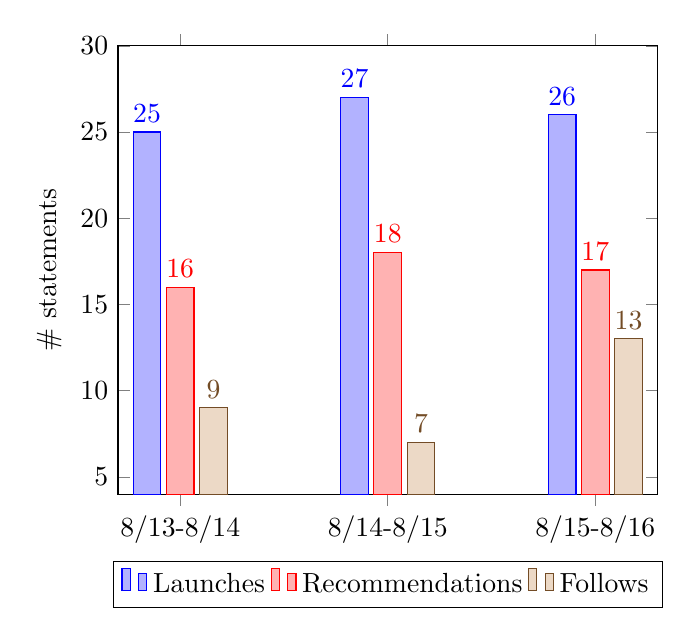
\begin{tikzpicture}
  \begin{axis}[
    ybar,
    enlargelimits=0.15,
    legend style={at={(0.5,-0.15)},
      anchor=north,legend columns=-1},
    ylabel={\# statements},
    symbolic x coords={8/13-8/14,8/14-8/15,8/15-8/16},
    xtick=data,
    nodes near coords,
    nodes near coords align={vertical},]
    \addplot coordinates {(8/13-8/14,25) (8/14-8/15,27) (8/15-8/16,26)};
    \addplot coordinates {(8/13-8/14,16) (8/14-8/15,18) (8/15-8/16,17)};
    \addplot coordinates {(8/13-8/14,9) (8/14-8/15,7) (8/15-8/16,13)};
    \legend{Launches,Recommendations,Follows}
  \end{axis}
\end{tikzpicture}
\begin{itemize}
\item The percentages described in section 5.9 are not displayed here.
\end{itemize}

\subsection{Prototype Improvement Suggestions}
Additional features may be implemented on top of this base
specification but they would require adding aditional values to each
subarray returned by the algorithm. These additional values can be
retrieved via (1) performing metadata lookup within or independently
of the algorithm (2) by utilizing additional xAPI statement paramters
and/or (3) by performing additional computations. The following
examples assume the metadata is contained within each statement
available to the algorithm.

\begin{itemize}
\item populate a tooltip with the most popular launched, recommended
  and followed activity.
\item populate a tooltip with the number of actors associated with the
  launches and follows.
\item populate a tooltip with the actor who most often and the actor
  who lease often follows recommendations.
\end{itemize}

\end{document}
